% --TODO: - Proyecto:
%    - Crear flujo de trabajo [X] - Johan
%    - Asignar temas y trabajos a cada uno [X] - Guena
%    - Crear y configurar el repositorio [X] - Guena

% --TODO: - Utilidades de LaTeX:
%    - Averiguar como implementar graficas y demas [X] - Johan

\documentclass[letterpaper,14pt]{extreport} % Modo Papel de carta, fuente de 14pt, formato de reporte

\usepackage[utf8]{inputenc}
\usepackage{amsmath}
\usepackage{amssymb}
\usepackage{ragged2e}
\usepackage{blindtext}
\usepackage{geometry}
\usepackage{enumitem}
\usepackage{float}
\usepackage{graphicx}
\usepackage{authblk}
\usepackage[
backend=biber,
style=alphabetic,
sorting=ynt
]{biblatex}

\addbibresource{ref.bib}

% --TODO: - Titulo:
%    - Dar formato al titulo [X] - Guena
%    - Poner correctamente los nombres de autor [X] - Guena
%    - Agregar la fecha oficial [X] - Guena

\title{Cambios de Coordenadas Rectangulares a Esféricas}
% --CHANGED: Agregados múltiples autores + afiliaciones (authblk)
\author[1]{Guennadi Maximov Cortés}
\author[2]{Johan Ulises Herrera Wences}
\affil[1,2]{Tecnologías de la Información en Ciencias, Universidad Nacional Autónoma de México}
\date{25/01/2022}

\renewcommand*\contentsname{Índice} % Da formato a la Tabla de Contenidos

% --FIXED: Elimina el texto "Chapter N"
\makeatletter
\def\@makechapterhead#1{
  \vspace*{50\p@}{\parindent\z@\raggedright\normalfont
  \ifnum\c@secnumdepth>\m@ne
    \if @mainmatter\Huge\bfseries\space\thechapter.\space
    \fi
  \fi
    \interlinepenalty\@M\Huge\bfseries#1\par\nobreak\vskip 40\p@
  }}
\makeatother


% --TODO: - Documento:
%    - Crear las secciones [X] - Guena
%    - Crear y formatear el texto []

\begin{document}

  \maketitle
  \pagenumbering{arabic}
  \tableofcontents
  \newpage

  \chapter{Introducción}
      En este documento se explicarán las coordenadas esféricas, sus propiedades, sus aplicaciones y cómo convertirlas a otros sistemas de coordenadas.


    \section{Abstracto}
      Las coordenadas esféricas se definen como:

\begin{eqnarray*}
  \overline{P} = \left(r,\theta,\varphi\right)
\end{eqnarray*}

Donde ${r}$ es la distancia del origen al punto, ${\theta}$ es el ángulo respecto al eje Z, y ${\varphi}$ es el ángulo respecto al eje X.

La conversión de coordenadas rectangulares a esféricas se define del siguiente modo:

% --TODO: Definir las conversiones.
\begin{eqnarray*}
  \left(x,y,z\right) = ...
\end{eqnarray*}

La conversión de coordenadas esféricas a rectangulares se define del siguiente modo:

% --TODO: Definir las conversiones.
\begin{eqnarray*}
  \left(r,\theta,\varphi\right) = ...
\end{eqnarray*}


  \chapter{Desarrollo}
    \renewcommand{\chaptername}{Jornada}

    \section{Introducción}
      Lorem ipsum...


      \subsection{¿Qué es una esfera?}
          Una esfera es una superficie tridimensional...


      \subsection{Ecuación de una esfera}
          La ecuación de la esfera se deriva de la ecuación de la circunferencia, a partir de su forma más simple:

\begin{eqnarray*}
  x^2+y^2=r^2
\end{eqnarray*}

Agregando un nuevo eje ${z}$ y, a su vez, agregando una coordenada ${z}$ a los puntos de la circunferencia, se crea un triángulo rectángulo imaginario conteniendo como catetos el radio de la circunferencia original y el valor de la coordenada ${z}$:

\begin{eqnarray*}
  r^2+z^2=R^2
\end{eqnarray*}

Si sustituimos el radio de la circunferencia por sus valores ${x}$ y ${y}$, tenemos:

\begin{eqnarray*}
  x^2+y^2+z^2=R^2
\end{eqnarray*}

En caso de un centro variable con coordenadas ${\left(h,k,l\right)}$, si aplicamos una transformación de traslación, tenemos la ecuación general de una esfera:

\begin{eqnarray*}
  \left(x-h\right)^2+\left(y-k\right)^2+\left(z-l\right)^2=R^2
\end{eqnarray*}

Si desarrollamos la ecuación anterior, llegamos a la forma general de una esfera:

\begin{eqnarray*}
  x^2+y^2+z^2+Ax+By+Cz+D=0
\end{eqnarray*}


      \subsection{¿Qué son las coordenadas esféricas?}
          Las coordenadas esféricas son un sistema de coordenadas en un sistema de 3 ejes ${\left(x,y,z\right)}$, donde todo punto es descrito con la siguiente notación:

\begin{eqnarray}
  \overline{P}=\left(r,\theta,\phi\right)
\end{eqnarray}

Donde ${r}$ es la distancia del punto al origen, ${\theta}$ es el ángulo que forma el segmento radial con el eje ${z}$, y ${\phi}$ es el ángulo que forma el segmento radial con el eje ${x}$.

Por convención, cada uno de los valores se confina en los siguientes rangos:

\begin{equation*}
  \begin{split}
    0\ \leq\ &r\ <\ \infty\\
    0\ \leq\ &\theta\ \leq\ \pi\\
    0\ \leq\ &\phi\ \leq\ 2\pi
  \end{split}
\end{equation*}


      \subsection{Gráfica de un punto en coordenadas esféricas}
          Como demostración, las gráficas de coordenadas polares se representan del siguiente modo:

% --TODO: Incluir gráfica genérica

A favor 


    \section{Conversión de coordenadas}
      Podemos establecer una relación entre las coordenadas rectangulares y las polares mediante la construcción de un punto $(x,y)$ en un plano bidimensional, como se muestra en la siguiente ilustración:

\begin{figure}[H]
  \centering
  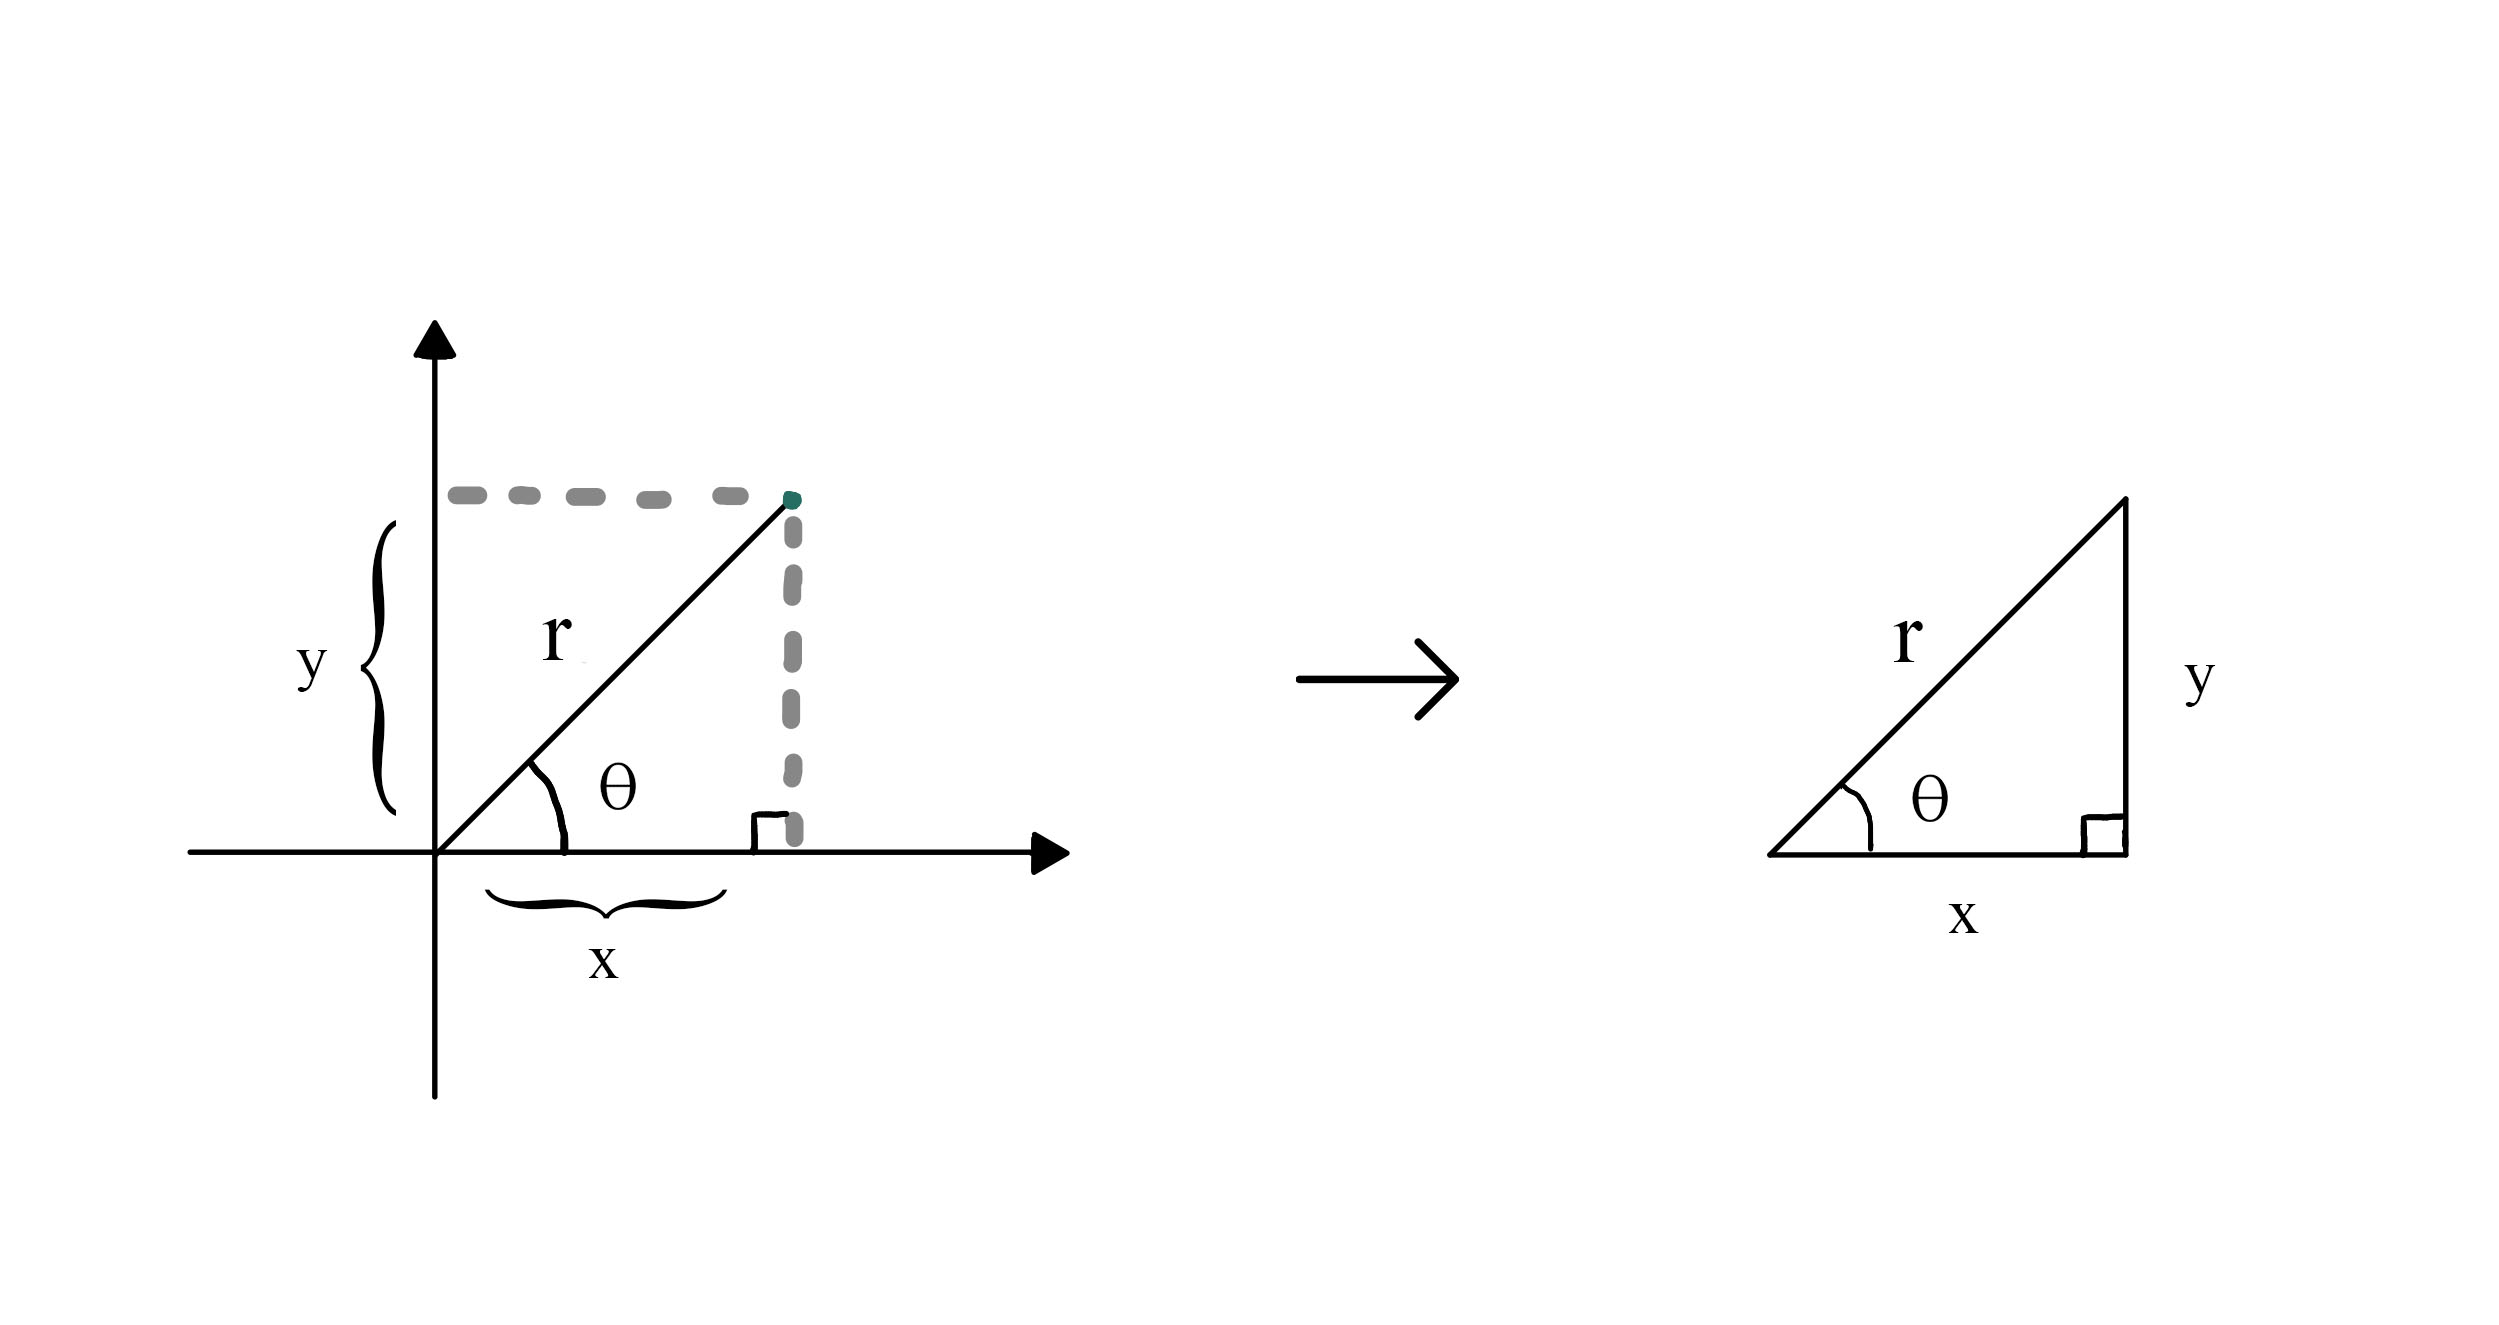
\includegraphics[width=11.17cm, height=5.67cm]{img/graph/relacion_r}
  \caption{Relación de coordenadas rectangulares y polares.}
  \label{relacion_de_coordenadas}
\end{figure}

Donde ${r}$ representa la distancia desde el origen hasta el punto y el ángulo es ${\theta}$. Por tanto, existe la coordenada polar ${\left(r,\theta\right)}$, donde el origen permanece igual y el eje polar se representa como el mismo eje x. De ésta manera, se forma un triángulo rectángulo y se tienen las siguientes relaciones:

\begin{eqnarray*}
  \cos\theta = \frac{\text{cateto adyacente}}{\text{hipotenusa}} = \frac{x}{r} &\rightarrow x = r\cos\theta\\\\
  \sin\theta = \frac{\text{cateto opuesto}}{\text{hipotenusa}} = \frac{y}{r} &\rightarrow y = r\sin\theta\\\\
  \tan\theta = \frac{\text{cateto opuesto}}{\text{cateto adyacente}} = \frac{y}{x} &\rightarrow \theta = \tan^{-1}\left(\frac{y}{x}\right)
\end{eqnarray*}

\vspace{4mm}
Dichas relaciones serán útiles cuando se intente establecer los métodos de transformación de coordenadas.


      \subsection{De coordenadas esféricas a rectangulares}
          Mediante la siguiente ilustración se observa el punto rojo en el espacio tridimensional con coordenadas esféricas ${\left(\rho,\theta,\varphi\right)}$, que proyecta un plano perpendicular al plano ${\left(x,y\right)}$, en dicho espacio se forman ${2}$ triángulos rectángulos. Es importante señalar que la variable ${r}$ es una coordenada polar que ayuda en la formación del triángulo rectángulo y su relación con las coordenadas ${\left(x,y\right)}$. Por ello, para el ángulo interno ${\varphi}$ se calcularán sus funciones trigonométricas.

\begin{figure}[H]
  \centering
  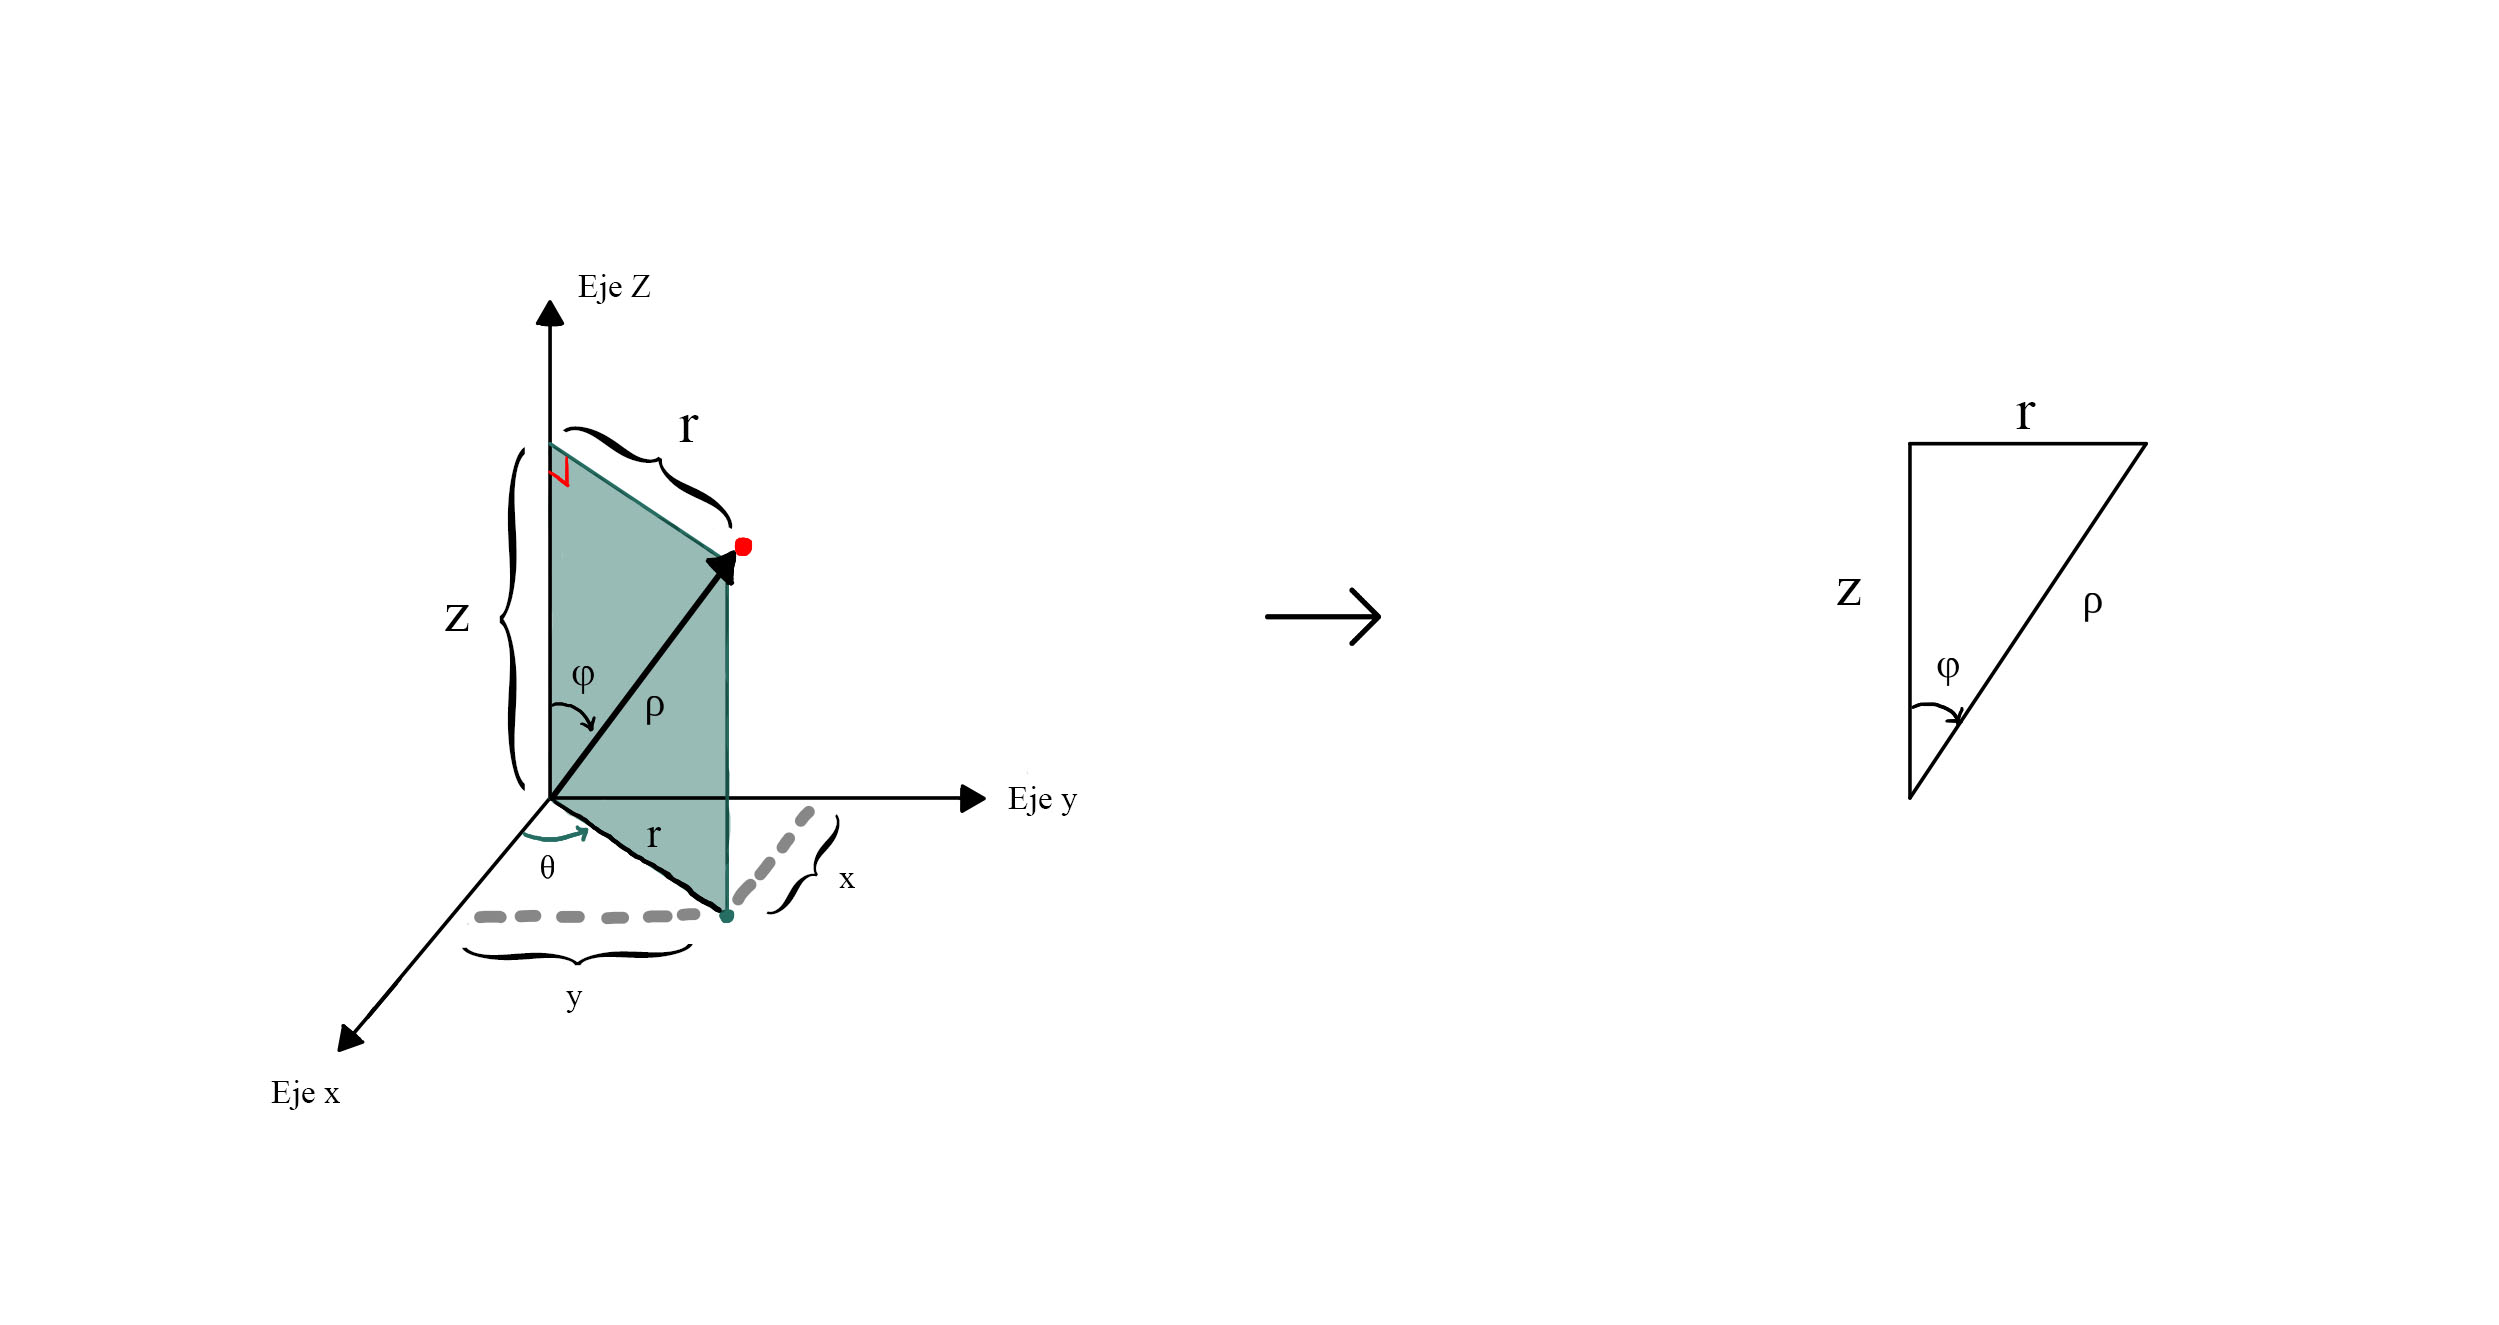
\includegraphics[width=11.17cm, height=5.67cm]{img/graph/coord_esf_2_rect_1.jpg}
  \caption{Triángulo rectángulo de un plano tridimensional.}
  \label{relacion_de_coordenadas}
\end{figure}

Entonces:
\begin{eqnarray*}
  \cos \varphi = \frac{\text{cateto adyacente}}{\text{hipotenusa}} = \frac{z}{\rho} \rightarrow z = \rho \cos \varphi\\\\
  \sin \varphi = \frac{\text{cateto opuesto}}{\text{hipotenusa}} = \frac{r}{\rho} \rightarrow r = \rho \sin \varphi
\end{eqnarray*}

\vspace{4mm}
Pero por la relación que se estableció con las coordenadas rectangulares y polares, entonces:

\begin{eqnarray*}
  x = r \cos \theta \rightarrow x = \rho \sin \varphi \cos \theta = \rho \cos \theta \sin \varphi\\\\
  y = r \sin \theta \rightarrow y = \rho \sin \varphi \sin \theta = \rho \sin \theta \sin \varphi
\end{eqnarray*}

\vspace{4mm}
Ahora, cuando se tienen coordenadas esféricas con el uso de dichas ecuaciones, se podrá determinar en el sistema de coordenadas $(x,y,z)$ (rectangulares).


          \subsubsection{Ejemplos prácticos de transformación de coordenadas esféricas a rectangulares}
          1) Convertir la coordenada $(6,\frac{\pi}{3},\frac{\pi}{6})$ esférica al sistema rectangular.

\begin{equation*}
  \begin{split}
    x = \rho \cos \theta \sin \varphi &= 6 \cdot \cos \left(\frac{\pi}{3}\right) \cdot \sin \left( \frac{\pi}{6} \right) = \frac{3}{2}\\
    y = \rho \sin \theta \sin \varphi &= 6 \cdot \sin \left( \frac{\pi}{3} \right) \cdot \sin \left(\frac{\pi}{6} \right) =\frac{3\sqrt{3}}{2}\\
    z = \rho \cos \varphi &= 6 \cdot \cos \left(\frac{\pi}{6} \right) = 3 \sqrt{3}
  \end{split}
\end{equation*}

\vspace{4mm}
2) Convertir la coordenada ${\left(0, \pi , \frac{\pi}{5}\right)}$ esférica al sistema rectangular.

\begin{equation*}
  \begin{split}
    x = \rho \cos \theta \sin \varphi &= 0 \cdot \cos \left(\pi\right) \cdot \sin \left(\frac{\pi}{5}\right) = 0\\
    y = \rho \sin \theta \sin \varphi &= 0 \cdot \sin \left(\pi \right) \cdot \sin \left(\frac{\pi}{5} \right) = 0\\
    z = \rho \cos \varphi &= 0 \cdot \cos \left(\frac{\pi}{5} \right) = 0
  \end{split}
\end{equation*}

\vspace{4mm}
3) Convertir la coordenada ${\left(3,0,\frac{\pi}{3} \right)}$ esférica al sistema rectangular.

\begin{equation*}
  \begin{split}
    x = \rho \cos \theta \sin \varphi = 3 \cdot \cos\left(0\right) \cdot \sin \left(\frac{\pi}{3}\right) &= 3 \cdot \left(1\right) \left(\frac{\sqrt{3}}{2} \right) = \frac{3\sqrt{3}}{2}\\
    y = \rho \sin \theta \sin \varphi = 3 \cdot \sin\left(0\right) \cdot \sin \left( \frac{\pi}{3} \right) &= 3 \cdot \left(0\right) \cdot \left(\frac{\sqrt{3}}{2}\right) = 0\\
    z = \rho \cos \varphi = 3 \cdot \cos \left( \frac{\pi}{3}\right) &= 3 \cdot \left(\frac{1}{2}\right) =\frac{3}{2}
  \end{split}
\end{equation*}

\vspace{4mm}
4) Convertir la coordenada ${\left(3, \frac{\pi}{3},0\right)}$ esférica al sistema rectangular.

\begin{equation*}
  \begin{split}
    x = \rho \cos \theta \sin \varphi = 3 \cdot \sin \left(\frac{\pi}{3}\right) \cdot \sin \left(0\right) &= 3 \cdot \left(\frac{1}{2}\right) \cdot \left(0\right) = 0\\
    y = \rho \sin \theta \sin \varphi = 3 \cdot \sin \left(\frac{\pi}{3}\right) \sin \left(0\right) &= 3 \cdot \left(\frac{\sqrt{3}}{2}\right) \cdot \left(0\right) = 0\\
    z = \rho \cos \varphi = 3 \cdot \cos\left(0\right) &= 3\left(1\right) = 3
  \end{split}
\end{equation*}


      \subsection{De coordenadas rectangulares a esféricas}
          Lorem ipsum dolor sit amet, consectetur adipisicing elit, sed do eiusmod tempor incididunt ut labore et dolore magna aliqua.


          \subsubsection{Ejemplos prácticos de transformación de coordenadas esféricas a rectangulares}
          1) Convertir la coordenada ${(1,2,2)}$ rectangular al sistema esférico.
\[\rho = \sqrt{x^{2}+y^{2}+z^{2}} = \sqrt{1^{2}+2^{2}+2^{2}} = 3\]
\[\varphi = cos^{-1}\left(\frac{z}{p}\right) = cos^{-1}\left(\frac{2}{3}\right) = 48.19^{\circ} = 0.84\]
\[\theta = tan^{-1}(2) = 63.43^{\circ} = 1.11\]

\vspace{4mm}
2) Convertir la coordenada ${(-2,2\sqrt{3},4)}$ rectangular al sistema esférico.
\[\rho = \sqrt{x^{2}+y^{2}+z^{2}} = \sqrt{(-2)^2+(2\sqrt{3})^{2}+4^{2}} = 4 \sqrt{2}\]
\[\varphi = cos^{-1}\left(\frac{4}{4\sqrt{2}}\right) = 45^{\circ} = \frac{\pi}{4}\]

\vspace{4mm}
Es importante analizar las coordenadas ${(x,y)}$, es decir ${(-2,2\sqrt{3})}$ para determinar su cuadrante y de esa manera saber cómo proceder en el proceso de obtención del valor de ${\theta}$. Como en éste caso, se encuentra en el segundo cuadrante, entonces no es útil el uso de la ecuación deducida anteriormente para encontrar ${\theta}$, sino determinar el ángulo complementario ${\alpha}$ y luego realizar la resta de dicho ángulo para determinar ${\theta}$, se puede visualizar en la siguiente imagen.

\begin{figure}[H]
  \centering
  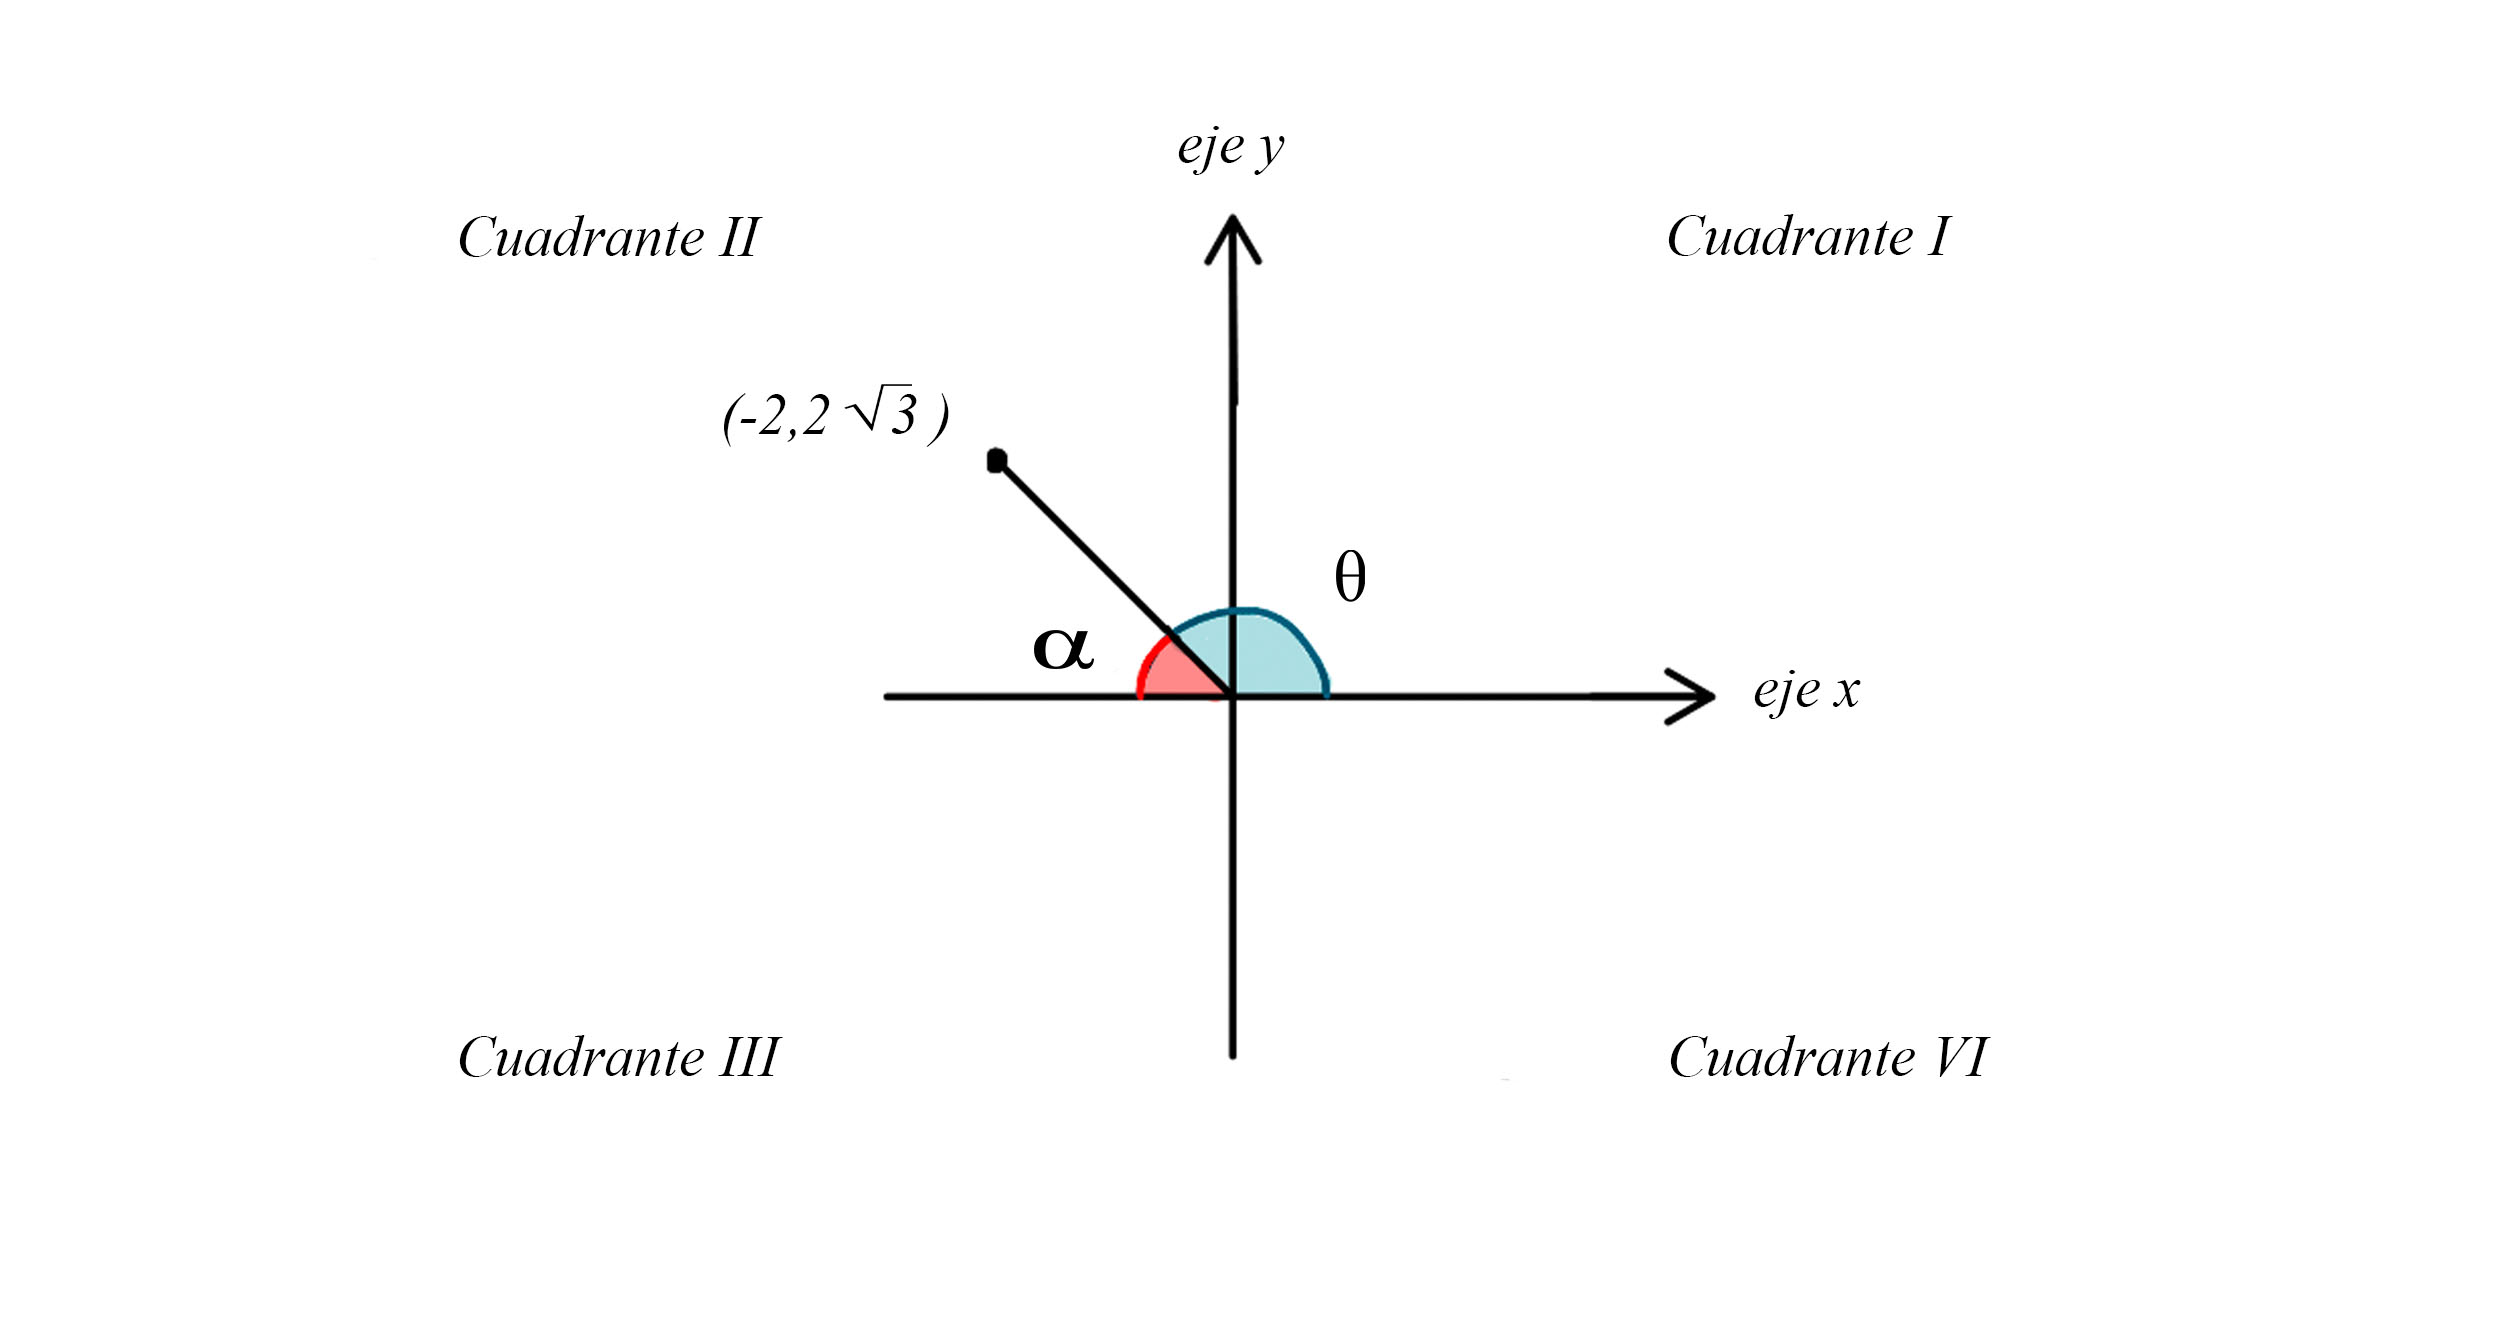
\includegraphics[width=11.17cm, height=5.67cm]{img/graph/segundo_cuadrante.jpg}
  \caption{Punto con coordenadas ${(-2,2\sqrt{3})}$.}
\end{figure}

Donde ${\alpha}$ representa el ángulo de interés para abordar su complemento ${\theta}$. Entonces, para encontrar el ángulo ${\alpha}$ se sabe que:
\[\alpha = tan^{-1}\left(\frac{y}{x}\right) = tan^{-1} \left( \left|\frac{2\sqrt{3}}{-2} \right| \right) = tan^{-1}(\sqrt{3}) = 60^{\circ} = \frac{\pi}{3} \]
\[\therefore \theta = 180^{\circ} - \alpha = 120^{\circ} =\frac{2\pi}{3}\]

\vspace{4mm}
3) Convertir la coordenada ${(-\sqrt{3},-1,-2\sqrt{3})}$ a su forma esférica.
\[\rho = \sqrt{x^{2}+y^{2}+z^{2}} = \sqrt{(-\sqrt{3})^{2}+(-1)^{2}+(-2\sqrt{3})^{2}} = 4\]
\[\varphi = cos^{-1}\left(\frac{z}{p}\right) = cos^{-1}\left(\frac{-2\sqrt{3}}{4}\right) = 150^{\circ} = \frac{5\pi}{6} \]

\vspace{4mm}
Nuevamente, primero calculamos el ángulo auxiliar ${\alpha}$ más cercano al eje x de las coordenadas ${(x,y) = (-\sqrt{3},-1)}$, como el punto se encuentra en el tercer cuadrante, entonces podremos realizar la suma del valor de ${\alpha}$ a ${180^{\circ}}$ para encontrar el valor de ${\theta}$.
\[\alpha = tan^{-1}\left(\frac{y}{x}\right) = tan^{-1}\left( \left|\frac{-1}{-\sqrt{3}}\right| \right) = 30^{\circ}\]
\[\therefore \theta = 180^{\circ} + \alpha = 210^{\circ} = \frac{7\pi}{6}\]


    \section{Conclusiones}
      \hspace{4mm} El uso de dichos sistemas de coordenadas en amplios campos del conocimiento refleja la utilidad del estudio de la localización de puntos en superficies esféricas. En cuando al uso de los distintos sistemas dependerá de la solución esperada en el desarrollo del problema que se esté tratando en particular. Tan sólo en la conversión de los distintos sistemas se encuentran ciertas dificultades en cada una de ellas. Por ejemplo, para convertir coordenadas de rectangulares a esféricas, en la obtención del ángulo ${\theta}$ se encuentra una ligera dificultad porque se necesita conocer la ubicación del punto y, en función de éste, encontrar el ángulo auxiliar más cercano al eje x que permita complementar la búsqueda del ángulo ${\theta}$. En cambio, utilizando coordenadas esféricas resulta trivial conocer los valores de sus equivalencias respecto al sistema rectangular. \cite{ecured}


  \medskip

  \printbibliography[title={Referencias}]

\end{document}
